\documentclass[11pt,a4paper]{article}

% These are extra packages that you might need for writing the equations:
\usepackage{amsmath}
\usepackage{amsfonts}
\usepackage{amssymb}
\usepackage{booktabs}
\usepackage{hyperref}
\usepackage{listings}
\usepackage{xcolor}
\usepackage{graphicx}
\usepackage{subcaption}

\lstset {language=C++,
		 basicstyle=\ttfamily,
         keywordstyle=\color{blue}\ttfamily,
         stringstyle=\color{red}\ttfamily,
         commentstyle=\color{purple}\ttfamily,
         morecomment=[l][\color{magenta}]{\#},
       	 basicstyle=\tiny}

% You need the following package in order to include figures in your report:
\usepackage{graphicx}

% With this package you can set the size of the margins manually:
\usepackage[left=2cm,right=2cm,top=2cm,bottom=2cm]{geometry}


\begin{document}

% Enter the exercise number, your name and date here:
\noindent\parbox{\linewidth}{
 \parbox{.25\linewidth}{ \large CSP, Exercise 03 }\hfill
 \parbox{.5\linewidth}{\begin{center} \large Beat Hubmann \end{center}}\hfill
 \parbox{.2\linewidth}{\begin{flushright} \large Mar 21, 2019 \end{flushright}}
}
\noindent\rule{\linewidth}{2pt}


\section{Introduction}

The Creutz algorithm~\cite{creutz} was implemented as another example of a Monte Carlo method to simulate
a microcanonical ('NVE') ensemble for the 3D Ising model. We focus our experiment on energy $E$ and calculate
temperature $T$ of the system from it in two different ways.

\section{Algorithm Description}
The implemented Creutz algorithm works as follows:
\begin{itemize}
	\item initialize 3d Ising grid with all spins aligned down.
	\item randomly pick a site: If flipping its spin increases total energy, do so;
	 repeat until system reaches target energy $E$
	\item release demon once system has reached target energy: Demon has energy $E_d=0$ with $E_{max}= 0.05\cdot E$. 
	\item demon jumps to random site and calculates $\Delta E$ for a potential spin flip: Iff $E_{max} \geq E_d \geq 0$ keep flip.
	\item recording $E_d$ completes one Monte Carlo step; repeat demon jump until number of steps required
\end{itemize}
The temperature $T$ then is calculated using two different ways for comparison:\\
The probability distribution $P(E_d)$ of the demon energy $E_d$ is plotted in a semilog plot.
The slope of the linear fit to $P(E_d)$ then equals the inverse temperature $\beta$ as in equation~\ref{eqn:1}.\\


\begin{equation}
	P(E_d) \approx e^{-\frac{E_d}{k_BT}}
\label{eqn:1}
\end{equation}

For comparison, the temperature is calculated analytically according to equation~\ref{eqn:2}.
\begin{equation}
	\frac{k_BT}{J} = \frac{4}{\log(1+\frac{4J}{<E_d>})}
\label{eqn:2}
\end{equation}


\section{Results}

The program was implemented as described above and submitted with this report. 
For all experiments, the coupling constant $J$ was fixed to the simplest ferromagnetic value of $J=1.0$. 
Experiments where run for system side lengths $L \in \{10, 20\}$ and average site energies $E \in \{-2.9, -2.5, -2.0, -1.5, -1.0, -0.5\}$ (figures~\ref{fig:1} and~\ref{fig:2}).

\begin{figure}[b]
	\centering
	\begin{subfigure}{.5\textwidth}
		\centering
		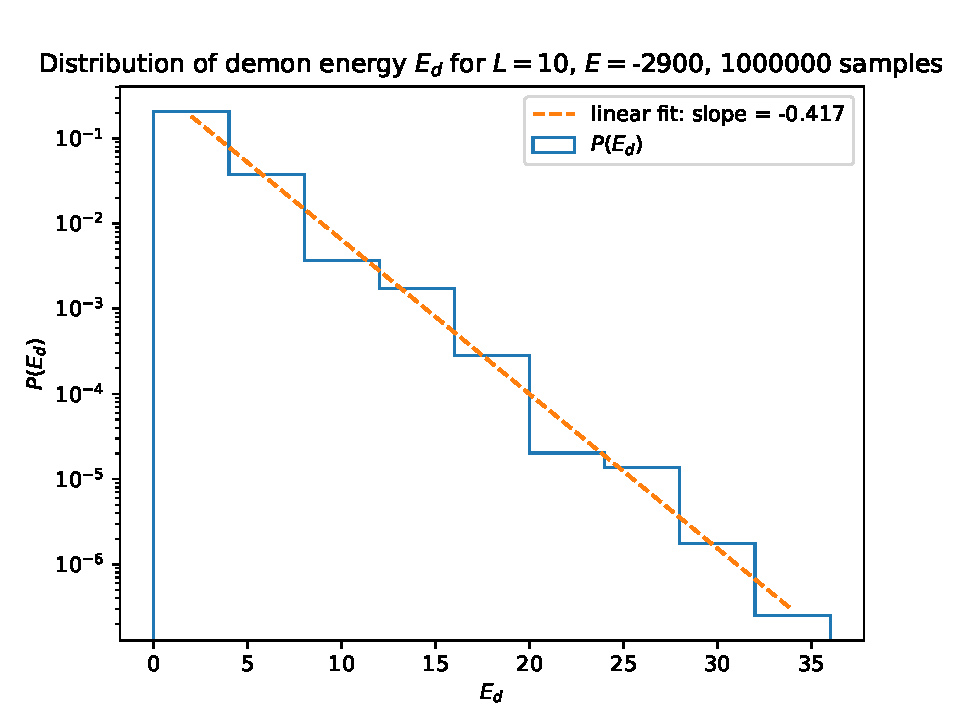
\includegraphics[width=0.9\textwidth]{E_d_L10_E2900.pdf}
	\end{subfigure}%
	\begin{subfigure}{.5\textwidth}
		\centering
		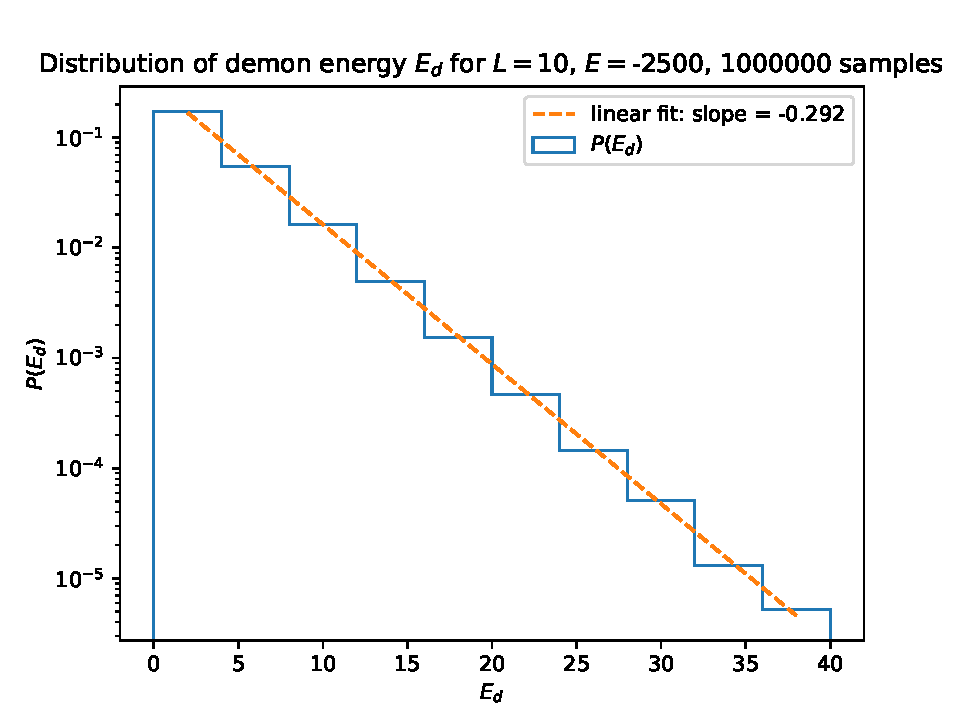
\includegraphics[width=0.9\textwidth]{E_d_L10_E2500.pdf}
	\end{subfigure}
	\begin{subfigure}{.5\textwidth}
		\centering
		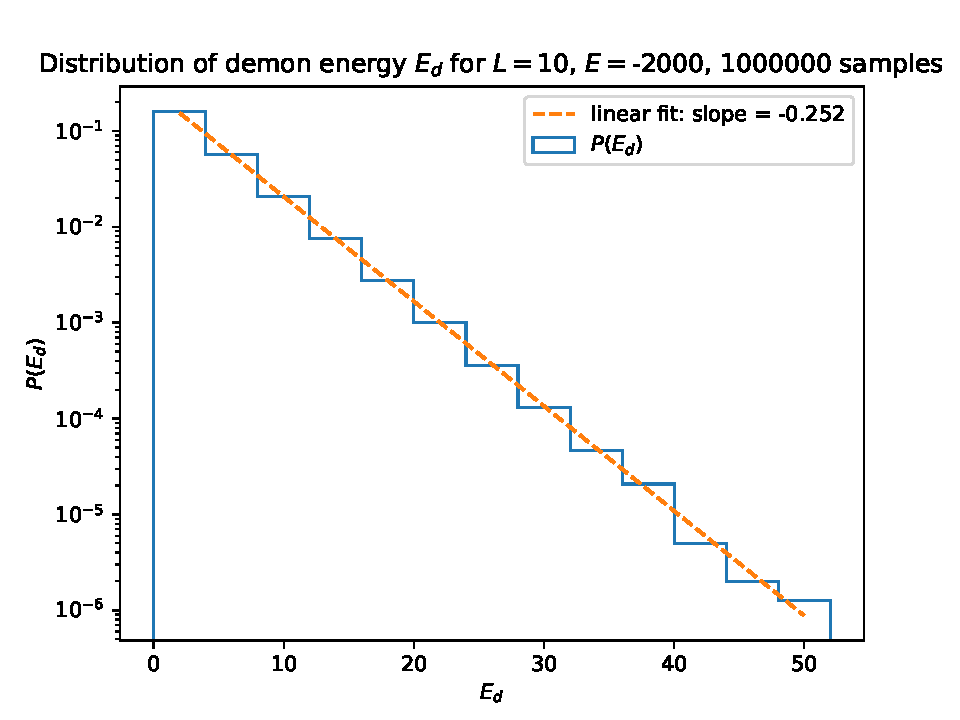
\includegraphics[width=0.9\textwidth]{E_d_L10_E2000.pdf}
	\end{subfigure}%
	\begin{subfigure}{.5\textwidth}
		\centering
		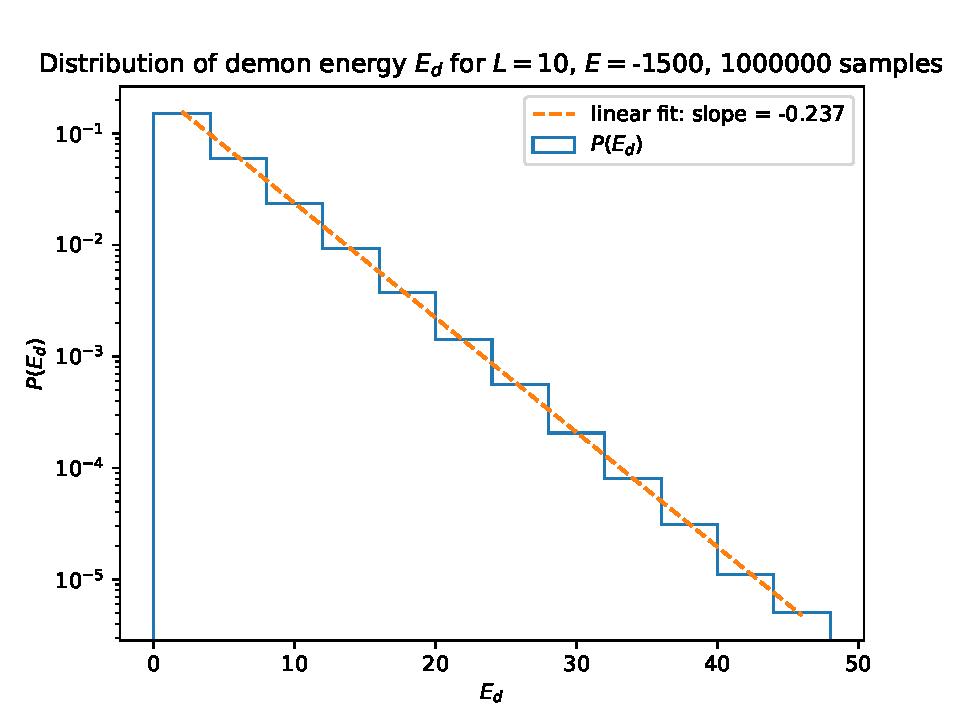
\includegraphics[width=0.9\textwidth]{E_d_L10_E1500.pdf}
	\end{subfigure}
	\begin{subfigure}{.5\textwidth}
		\centering
		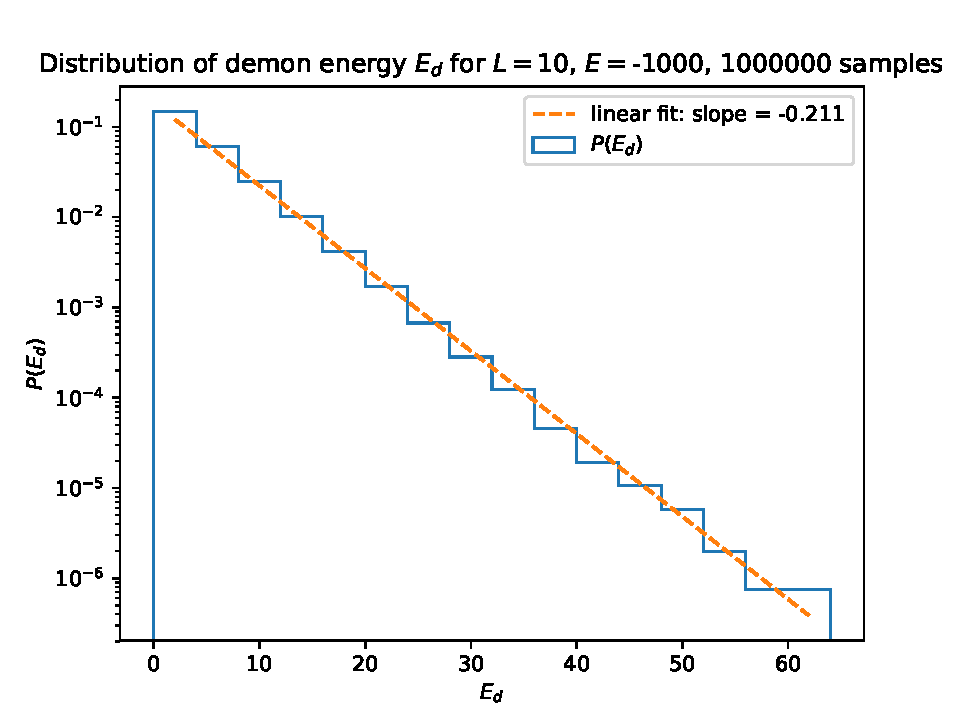
\includegraphics[width=0.9\textwidth]{E_d_L10_E1000.pdf}
	\end{subfigure}%
	\begin{subfigure}{.5\textwidth}
		\centering
		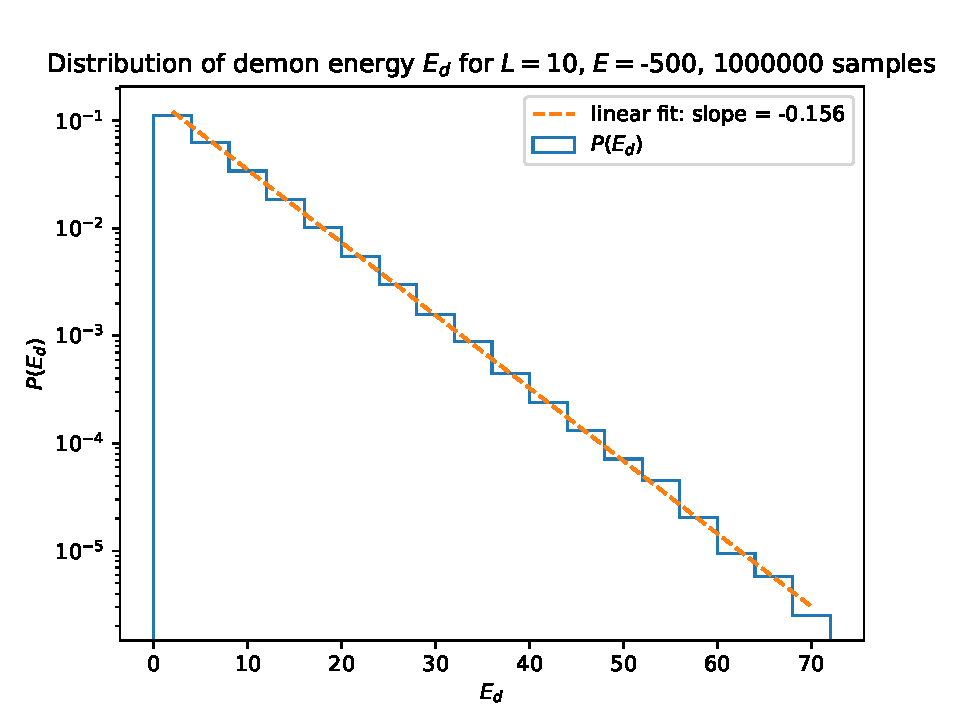
\includegraphics[width=0.9\textwidth]{E_d_L10_E500.pdf}
	\end{subfigure}
	\caption[short]{$P(E_d)$ plots for $L=10$}
	\label{fig:1}
	\end{figure}



	\begin{figure}[b]
		\centering
		\begin{subfigure}{.5\textwidth}
			\centering
			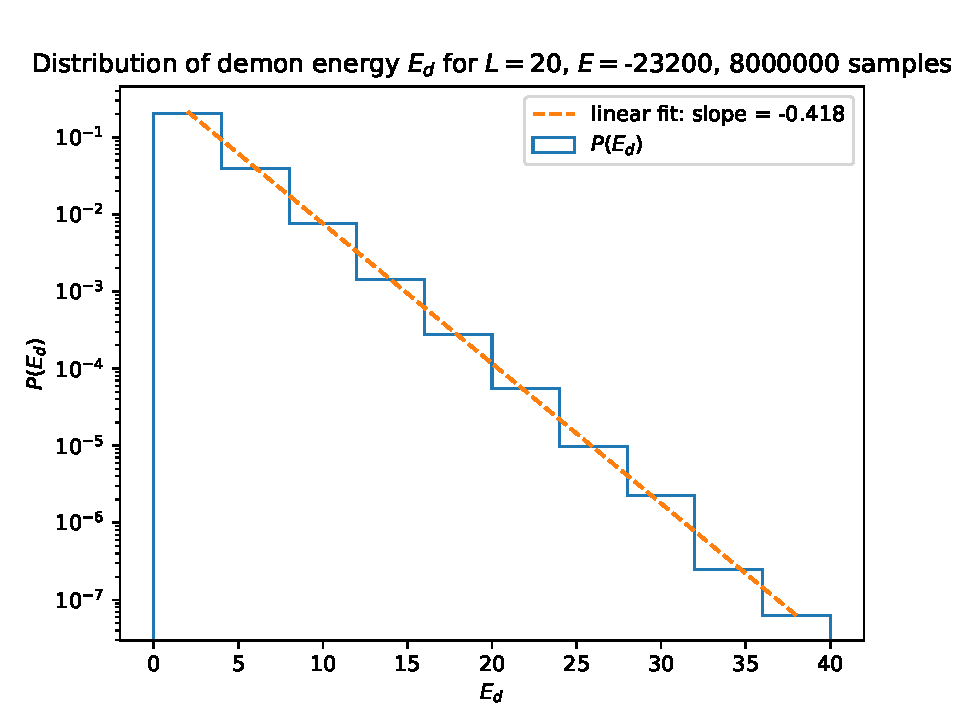
\includegraphics[width=0.9\textwidth]{E_d_L20_E23200.pdf}
		\end{subfigure}%
		\begin{subfigure}{.5\textwidth}
			\centering
			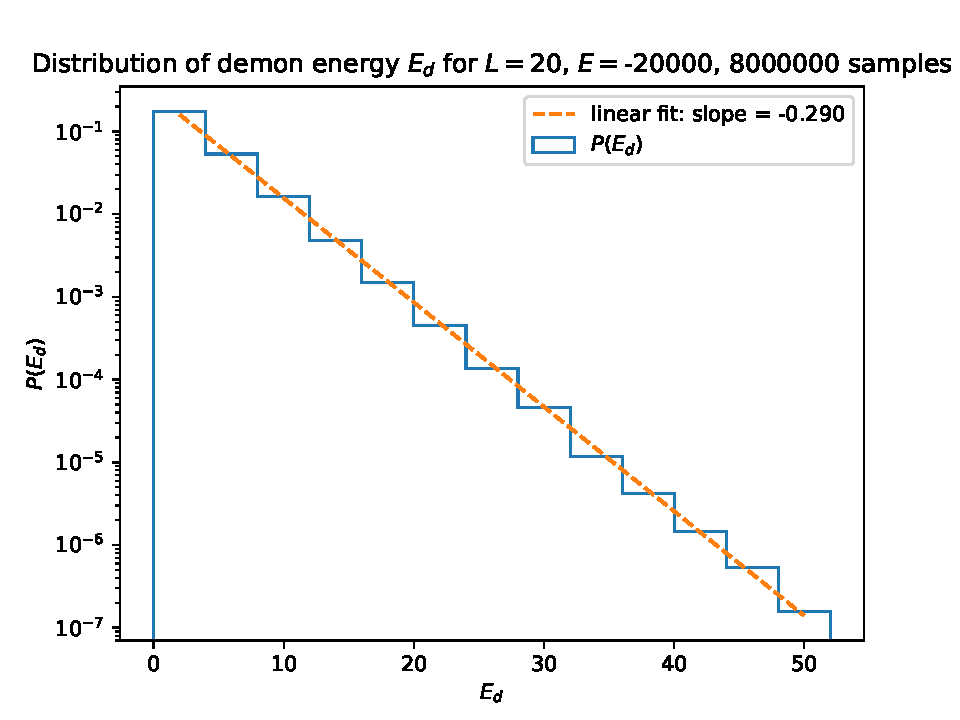
\includegraphics[width=0.9\textwidth]{E_d_L20_E20000.pdf}
		\end{subfigure}
		\begin{subfigure}{.5\textwidth}
			\centering
			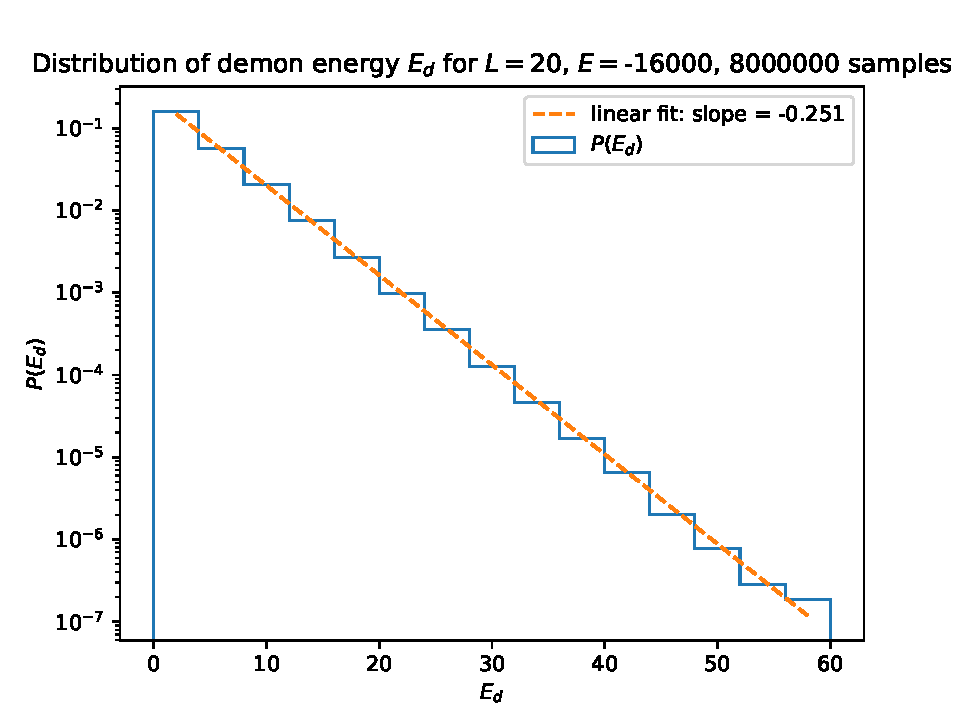
\includegraphics[width=0.9\textwidth]{E_d_L20_E16000.pdf}
		\end{subfigure}%
		\begin{subfigure}{.5\textwidth}
			\centering
			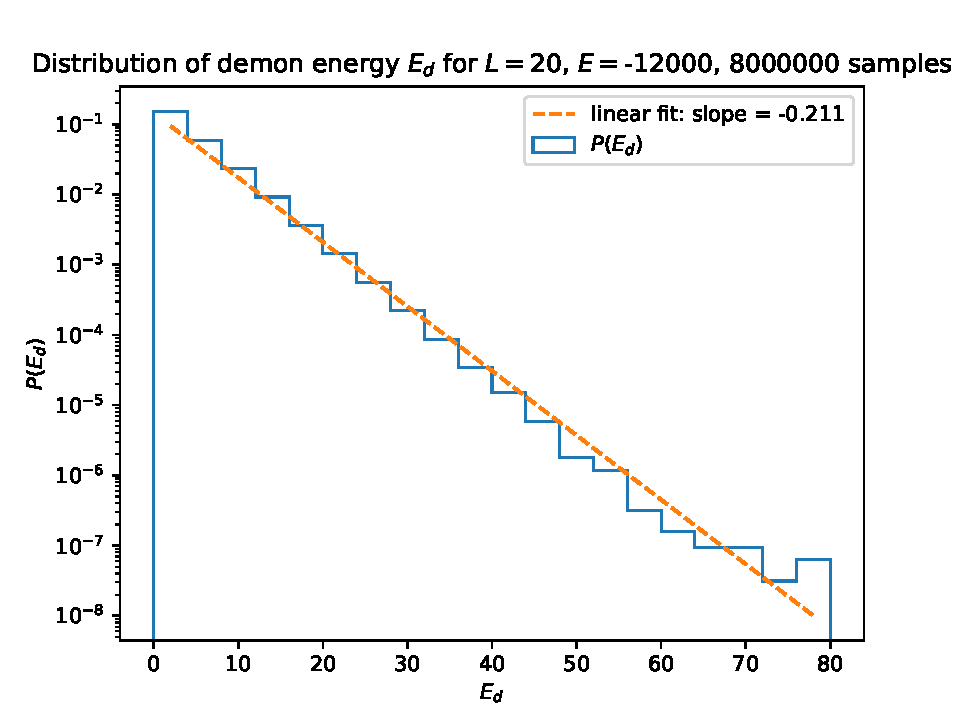
\includegraphics[width=0.9\textwidth]{E_d_L20_E12000.pdf}
		\end{subfigure}
		\begin{subfigure}{.5\textwidth}
			\centering
			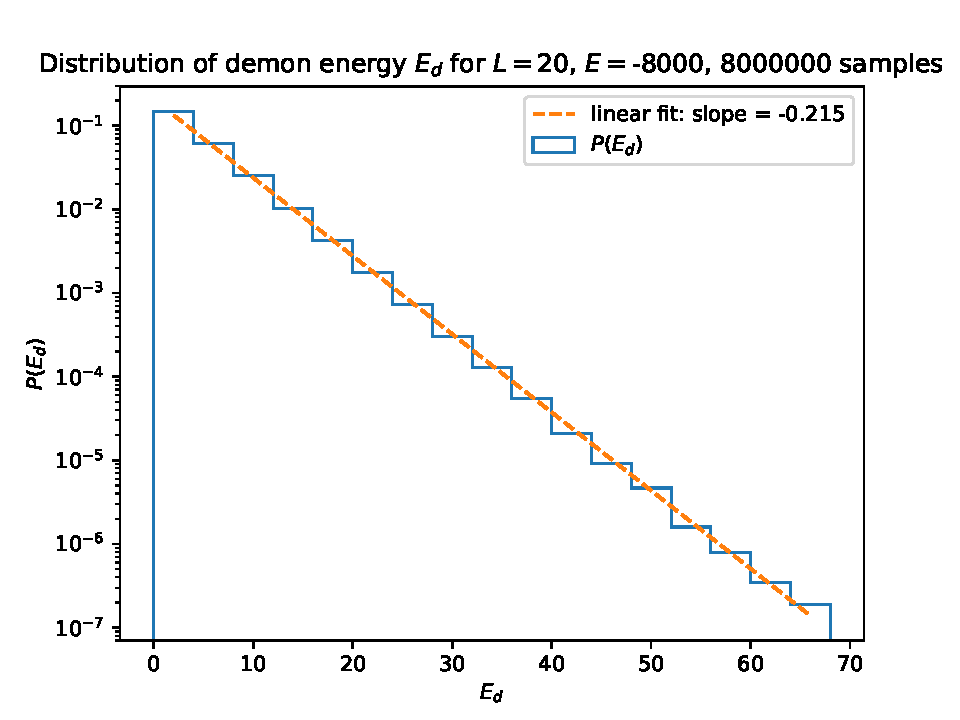
\includegraphics[width=0.9\textwidth]{E_d_L20_E8000.pdf}
		\end{subfigure}%
		\begin{subfigure}{.5\textwidth}
			\centering
			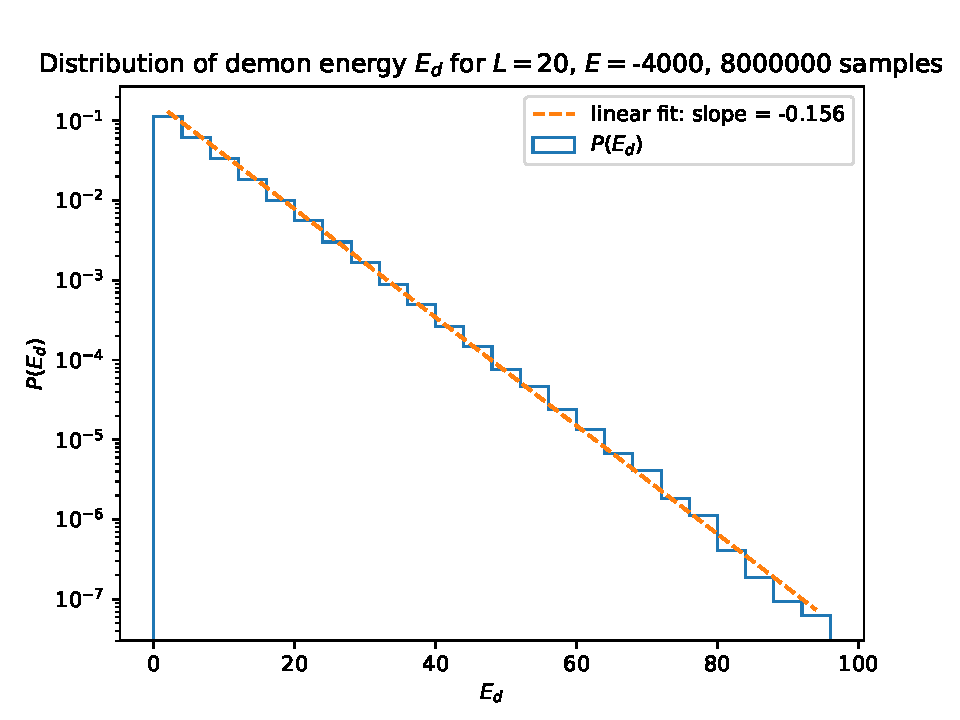
\includegraphics[width=0.9\textwidth]{E_d_L20_E4000.pdf}
		\end{subfigure}
		\caption[short]{$P(E_d)$ plots for $L=20$}
		\label{fig:2}
		\end{figure}
	
Calculated temperatures and plotted temperatures then were plotted for all energies (figures~\ref{fig:3} and~\ref{fig:4}).

\begin{figure}
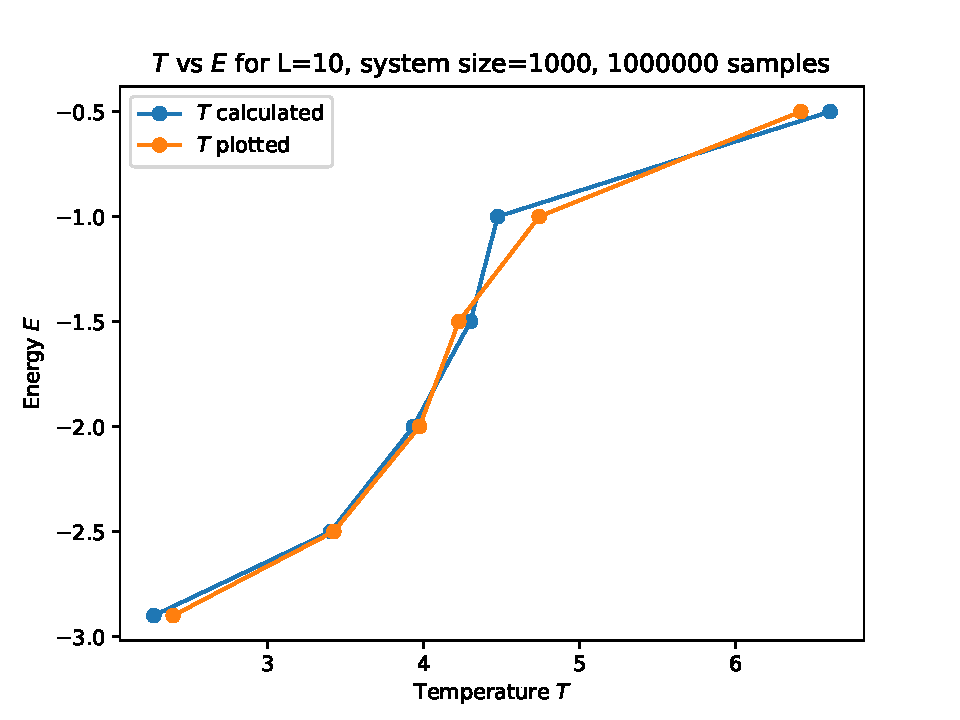
\includegraphics{T_vs_E_L10.pdf}
\caption{$T$ calculated and plotted versus $E$ for $L=10$.}
\label{fig:3}
\end{figure}

\begin{figure}
	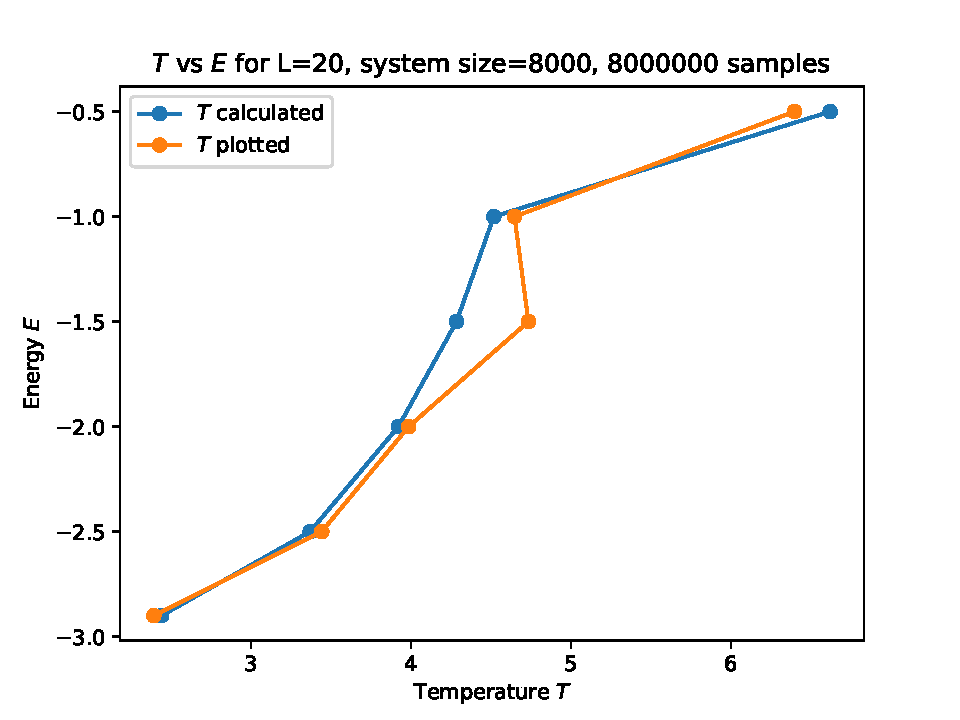
\includegraphics{T_vs_E_L20.pdf}
	\caption{$T$ calculated and plotted versus $E$ for $L=20$.}
	\label{fig:4}
	\end{figure}
	




\section{Discussion}
The results for dimensionless temperature $T$ agree almost perfectly between the two calculation methods.\\
Also, plotting temperatures for several energies in a single plot manages to reproduce the behaviour simulated using the 
Metropolis algorithm during a previous exercise (figures~\ref{fig:3} and~\ref{fig:4}).


\pagebreak
\begin{thebibliography}{99}

\bibitem{creutz}
	Creutz, M.\\
	\emph{Microcanonical Monte Carlo Simulation},\\
	Phys. Rev. Lett. American Physical Society. 50 (19): 1411–1414,\\
	1983.

% \bibitem{herrmann}
% 	Herrmann, H. J.,
% 	Singer, H. M.,
% 	Mueller L.,
% 	Buchmann, M.-A.,\\
% 	\emph{Introduction to Computational Physics - Lecture Notes},\\
% 	ETH Zurich,\\
% 	2017.

\bibitem{boettcher}
	Boettcher, L.,\\
	\emph{Computational Statistical Physics - Lecture Notes},\\
	ETH Zurich,\\
	2019.

\end{thebibliography}

\end{document}